\documentclass{article}

\usepackage{../preamble}
\standalonetrue

\pagestyle{fancy}
\fancyhf{}
\rhead{Section \thesection}
\lhead{PHYS 304 Lecture 07}
\rfoot{Page \thepage}


\title{PHYS 304 Lecture 07}
\author{Ashtan Mistal}
\date{!!!}

\begin{document}

\ifstandalone
\maketitle
\fi

\graphicspath{{./Lecture07/}}

\section{Key review of points from last day}

\begin{itemize}
    \item Explored the dynamical behaviour of an infinite square well wavefunction that is initially composed of an equally weighted simple sum of the two lowest stationary eigen states.
    \item Found that the associated probability density “sloshed” periodically back and forth from side to side, with a frequency 3 times the ground state eigen frequency, “bouncing off the walls”.  The period corresponds to the difference in eigen frequency between the two lowest level stationary states (essentially a beating effect). 
    \item Determined that the expectation value of the momentum oscillated at the same frequency, and this “made sense” (had the right relative phase with respect to the motion of $|\Psi(x,t)|^2$).
\end{itemize}

\textbf{Important note:}

The expectation value of momentum is \textit{not zero}, and it \textit{depends on time}. This is because our initial state is not proportional to a single eigenfunction of the time-independent Schrodinger equation, it therefore must be expanded in more than a single eigen function. 


\section{Harmonic Oscillator Potential}

\subsection{Activity 1}

What is $x(t)$ for a classical particle of mass $m$ initially at rest at a position $x = x_0$ in a harmonic potential $V = \frac{1}{2} kx^2$?

$$m \frac{d^2 x}{dt^2} = -kx \text{, since } F = - \nabla V = -kx$$

$$\frac{d^2 x}{dt^2} + \frac{k}{m} = 0 \Rightarrow x(t) = A \cos \left( \sqrt{\frac{k}{m}} t \right) + B \sin \left( \sqrt{\frac{k}{m}} t \right)$$

$x(0) = -x_0$, and $\frac{dx}{dt}(0) = 0$, therefore $A = -x_0$ and $B = 0$, giving us the following equation:

$$x(t) = -x_0 \cos \left( \sqrt{\frac{k}{m}} t \right)$$

What is the maximum distance it ever travels away from the origin?
$$x_0$$

\subsection{Activity 2}

What is the probability distribution, $P(x)$, for finding the particle at any positon $x$ (this is strictly a classical mechanics problem)?


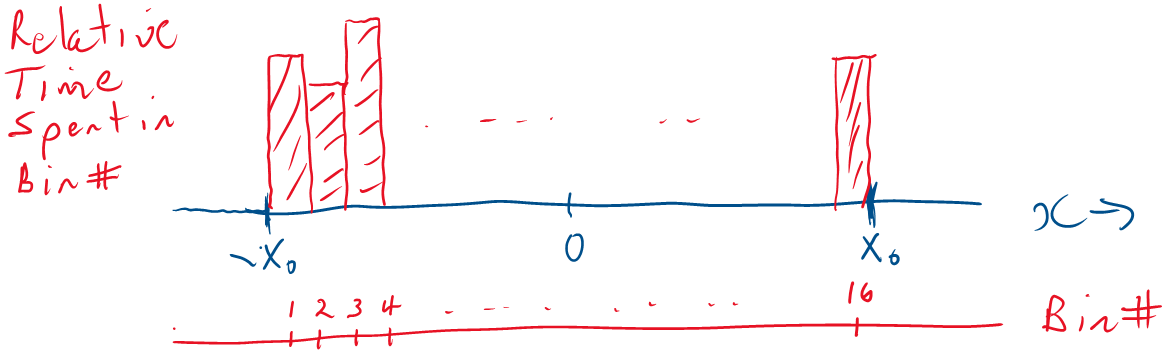
\includegraphics[width = 0.9 \textwidth]{Lecture07/1.png}

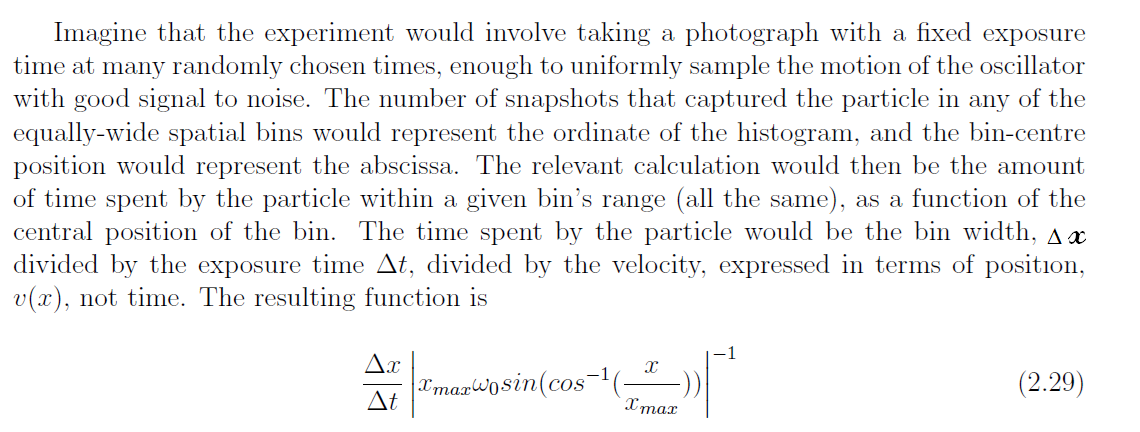
\includegraphics[width = 0.9 \textwidth]{Lecture07/2.png}

$$x(t) = -x_0 \cos \left( \sqrt{\frac{k}{m}} t \right)$$

Dwell time = $dx \frac{dt}{dx} = \frac{dx}{v(x)}$, we need to get $v(x)$, not $v(t)$. 

Plot from \verb|Harmonic_oscillator.py|:

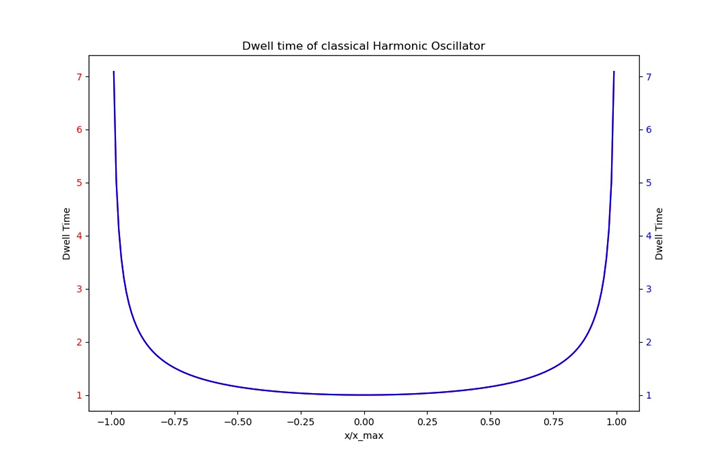
\includegraphics[width = 0.7 \textwidth]{Lecture07/3.png}

It is non-zero everywhere, spends more time near extremities. 


\subsection{Activity 3}

What is the full Schrodinger equation and the time independent Schrodinger equation for a quantum mechanical particle in this potential? Use dimensionless variables. 

$$i \hbar \frac{\partial \Psi(x,t)}{\partial t} = \left( - \frac{\hbar^2}{2m} \frac{\partial^2}{\partial x^2} + \frac{1}{2} kx^2 \right) \Psi(x,t)$$

where $\sqrt{\frac{k}{m}} = \omega$. 

$$\left(-\frac{\hbar^{2}}{2 m} \frac{d^{2}}{d x^{2}}+\frac{1}{2} m \omega_{0}^{2} x^{2}\right) \psi(x)=E \psi(x)$$


Render Dimensionless: $$E \rightarrow  \frac{E}{\hbar \omega_{0}} \cong K $$


$$\left(-\frac{\hbar}{2 m \omega_{0}} \frac{d^{2}}{d x^{2}}+\frac{1}{2} \frac{m \omega_{0}}{\hbar} x^{2}\right) \psi(x) = K \psi(x)$$

We also redefine $x \rightarrow \xi = \sqrt{\frac{m \omega_0}{2 \hbar}} \Rightarrow$

$$\left( - \frac{1}{4} \frac{d^2}{d \xi^2} + \xi^2 \right) \psi(\xi) = K \psi(\xi)$$

This is slightly untidy, so ket $K = \frac{2E}{\hbar \omega_0}$, and so

$$\left(- \frac{d^2}{d \xi^2} + \xi^2 \right) \psi(\xi) = K \psi(\xi), \text{ or }$$

$$\frac{d^2}{d \xi^2} \psi(\xi) = \left(\xi^2 - K \right) \psi(\xi)$$



\section{Analytic, brute force solution}

\textit{(See posted notes on Canvas and text for the more elegant solution)}

Four crucial steps from the dimensionless TISE, $\frac{d^2 \psi(\xi)}{d \xi^2} = (\xi - K) \psi(\xi)$, to determining the allowed energy levels and eigen functions:

\begin{enumerate}
    \item Find the function that satisfies the differential equation at large $\xi$, namely $e^{\pm \frac{\xi^{2}}{2}}$ and then let $\psi(\xi)=h(\xi) e^{-\frac{\xi^{2}}{2}}$
    \item Substitute this back into the full TISE and get a new differential equation for $h(\xi)$, namely $\frac{d^{2} h(\xi)}{d \xi^{2}}-2 \xi \frac{d h(\xi)}{d \xi}+(K-1) h(\xi)=0$
    \item Assume a power series expansion for $h(\xi), h(\xi)=\sum_{j=0}^{\infty} a_{j} \xi^{j}$, equate coefficients of each power of $\xi$, to arrive at a recursion relationship: $a_{j+2}=\frac{(2 j+1-K)}{(j+1)(j+2)} a_{j}$
    
    \item Use the boundary conditions that wave function has to go to zero at $+/$ - infinity to realize that allowed solutions are defined by some maximum value of $j$, call it $\mathrm{n}$, for which all higher expansion coefficients of $h(\xi)$ are zero.
\end{enumerate}

We have two key implications:

\begin{enumerate}
    \item From the recursion relation, for the power series to terminate means $K = K_n = 2n+1$ with $n=0,1,2,...$, which directly gives the allowed eigen energies as $E_n = \hbar \omega(n + \frac{1}{2})$. 
    
    \item The corresponding eigen functions then come in two flavours, odd and even with respect to x, given, to within a normalization factor, by choosing an n (either odd or even), then using the recursion relations with the corresponding value of $K_n$, starting with either $a_0 = 0, a_1 = 1$, for odd solutions, of $a_1 = 0, a_0 = 1$ for even solutions. 
\end{enumerate}


\subsection{Quantitatively}

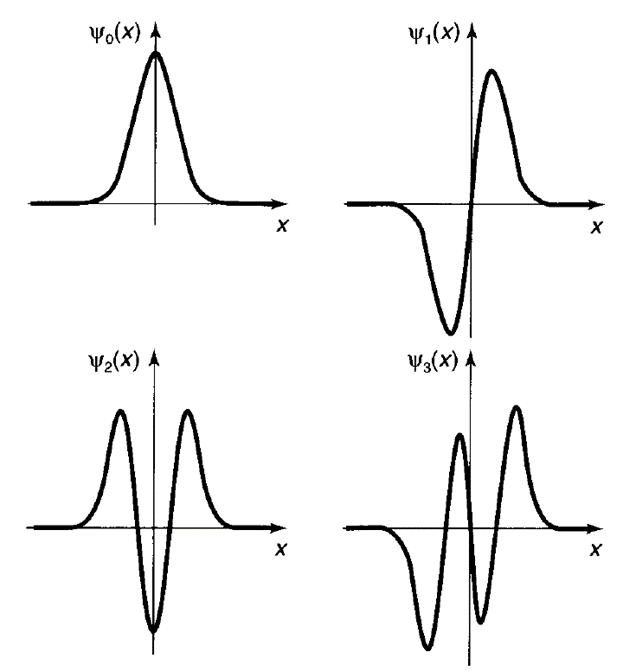
\includegraphics[width = 0.4 \textwidth]{Lecture07/4.png} 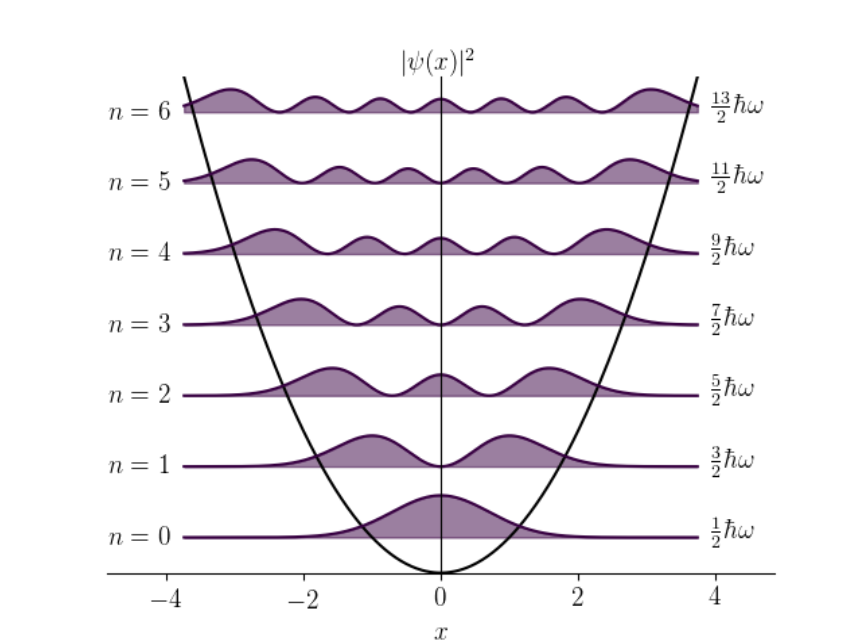
\includegraphics[width = 0.4 \textwidth]{Lecture07/5.png}

\hfill

What features of of this wavefunction imply “non-classical” behaviour of the quantum mechanical  particle in one of the lowest stationary states?

\begin{itemize}
    \item Extends beyond classical limits +/- x0
    \item Probability of finding it at certain positions is zero
\end{itemize}

What features of these HO solutions differ and which are similar to the infinite square well stationary solutions?


\begin{itemize}
    \item Quantized energy levels are similar
    \item Number of nodes = n
    \item Separation of energy levels different
    \item Separation of nodes not exactly periodic
\end{itemize}

\subsubsection*{In what limit do the eigen states look “almost classical”? }

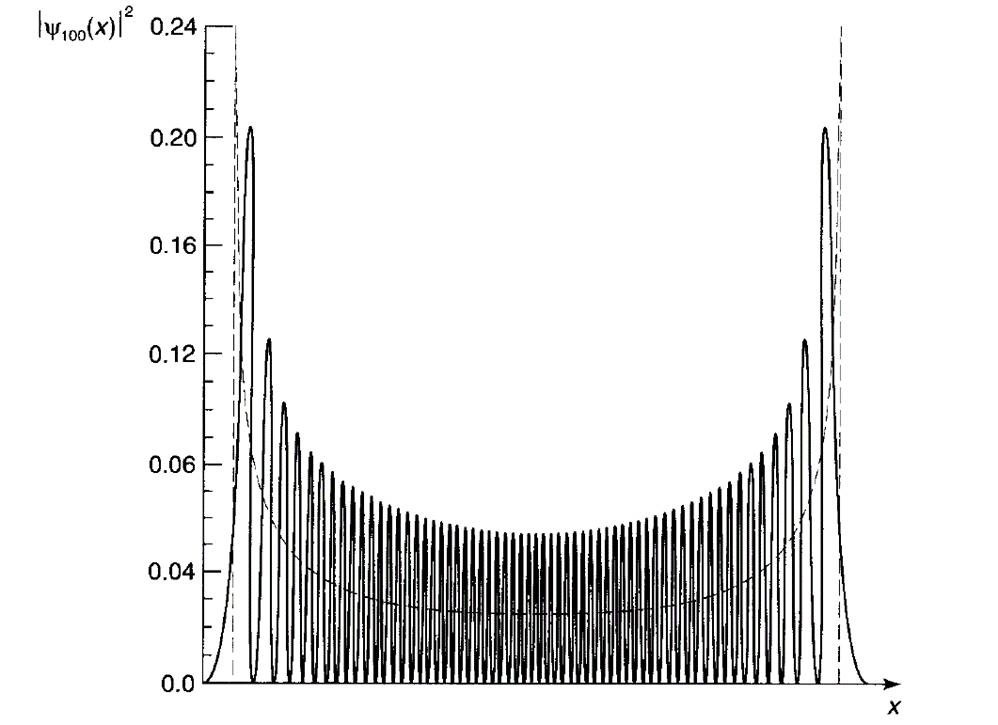
\includegraphics[width = 0.6 \textwidth]{Lecture07/6.png} 



\end{document}